\documentclass[12pt, a4paper]{report}
\usepackage{graphicx} % For including images
\usepackage{float} % For [H] table placement (prevents floating)
\usepackage{titlesec} % For customizing section titles
\usepackage{tocloft} % For customizing table of contents
\usepackage{acro} % For acronyms
%% ____Bibliography____%%
\usepackage[numbers,sort&compress]{natbib}
% chapterbib is for per-chapter bibliographies; this document uses one global bibliography.
% Keeping chapterbib enabled can interfere with citation resolution.
%\usepackage{chapterbib}
\usepackage[breaklinks]{hyperref} % For clickable links in the document
\hypersetup{
    hidelinks
}
%\hypersetup{colorlinks=true,citecolor=blue,linkcolor=blue,urlcolor=blue}
% Page margins
\usepackage[left=1.5in, right=1in, top=1in, bottom=1in]{geometry}

% Remove page number from the first page
\thispagestyle{empty}

% Customize table of contents, list of figures, and list of tables
\renewcommand{\cfttoctitlefont}{\hfill\Large\bfseries}
\renewcommand{\cftaftertoctitle}{\hfill}
\renewcommand{\cftloftitlefont}{\hfill\Large\bfseries}
\renewcommand{\cftafterloftitle}{\hfill}
\renewcommand{\cftlottitlefont}{\hfill\Large\bfseries}
\renewcommand{\cftafterlottitle}{\hfill}

% Define acronyms
\DeclareAcronym{ACC}{
  short = ACC,
  long  = Adaptive Cruise Control
}

\DeclareAcronym{ADAS}{
  short = ADAS,
  long  = Advanced Driver Assistance Systems
}

\DeclareAcronym{AI}{
  short = AI,
  long  = Artificial Intelligence
}

\DeclareAcronym{AV}{
  short = AV,
  long  = Autonomous Vehicle
}

\DeclareAcronym{CAN}{
  short = CAN,
  long  = Controller Area Network
}

\DeclareAcronym{CARLA}{
  short = CARLA,
  long  = Car Learning to Act
}

\DeclareAcronym{CNN}{
  short = CNN,
  long  = Convolutional Neural Network
}

\DeclareAcronym{DRL}{
  short = DRL,
  long  = Deep Reinforcement Learning
}

\DeclareAcronym{ECU}{
  short = ECU,
  long  = Electronic Control Unit
}

\DeclareAcronym{EV}{
  short = EV,
  long  = Electric Vehicle
}

\DeclareAcronym{FSD}{
  short = FSD,
  long  = Full Self-Driving
}

\DeclareAcronym{FOV}{
  short = FOV,
  long  = Field of View
}

\DeclareAcronym{GPS}{
  short = GPS,
  long  = Global Positioning System
}

\DeclareAcronym{HIL}{
  short = HIL,
  long  = Hardware-in-the-Loop
}

\DeclareAcronym{HPC}{
  short = HPC,
  long  = High-Performance Computing
}

\DeclareAcronym{ISO}{
  short = ISO,
  long  = International Organization for Standardization
}

\DeclareAcronym{LCA}{
  short = LCA,
  long  = Lane Centring Assistance
}

\DeclareAcronym{LCC}{
  short = LCC,
  long  = Lane Centring Control
}

\DeclareAcronym{LiDAR}{
  short = LiDAR,
  long  = Light Detection and Ranging
}

\DeclareAcronym{LKA}{
  short = LKA,
  long  = Lane Keeping Assistant
}

\DeclareAcronym{ML}{
  short = ML,
  long  = Machine Learning
}

\DeclareAcronym{MPC}{
  short = MPC,
  long  = Model Predictive Control
}

\DeclareAcronym{ODD}{
  short = ODD,
  long  = Operational Design Domain
}

\DeclareAcronym{PID}{
  short = PID,
  long  = Proportional-Integral-Derivative
}

\DeclareAcronym{RADAR}{
  short = RADAR,
  long  = Radio Detection and Ranging
}

\DeclareAcronym{RL}{
  short = RL,
  long  = Reinforcement Learning
}

\DeclareAcronym{ROS}{
  short = ROS,
  long  = Robot Operating System
}

\DeclareAcronym{SAE}{
  short = SAE,
  long  = Society of Automotive Engineers
}

\DeclareAcronym{SOTIF}{
  short = SOTIF,
  long  = Safety of the Intended Functionality
}

\DeclareAcronym{TEB}{
  short = TEB,
  long  = Timed Elastic Band
}

\DeclareAcronym{TTC}{
  short = TTC,
  long  = Time to Collision
}

\DeclareAcronym{V2I}{
  short = V2I,
  long  = Vehicle-to-Infrastructure
}

\DeclareAcronym{V2V}{
  short = V2V,
  long  = Vehicle-to-Vehicle
}

\begin{document}


\thispagestyle{empty}

\begin{center}

\begin{center}
 
\includegraphics[width=2cm,keepaspectratio=true]{uor_logo.jpg}
 % uor_logo.jpg: 236x331 pixel, 72dpi, 8.33x11.68 cm, bb=0 0 236 331
\end{center}

\vspace{1.5cm}
\begin{huge}
%%%%%%%%%%%%%%%%%%%%%%%%%%%%%%%%%%%%%%%%%%%%%%%%%%%%
% Project title
%%%%%%%%%%%%%%%%%%%%%%%%%%%%%%%%%%%%%%%%%%%%%%%%%%%%
AI-Driven Level 2 Driver Assistance for \\
\vspace{0.3cm}
Electric Vehicles
%%%%%%%%%%%%%%%%%%%%%%%%%%%%%%%%%%%%%%%%%%%%%%%%%%%%
\end{huge} \\
\vspace{1cm}

\begin{normalsize}
An undergraduate project proposal report submitted to the
\end{normalsize}\\
\vspace{1cm}

\begin{large}
Department of Computer Engineering\\
Faculty of Engineering\\
University of Ruhuna\\
Sri Lanka
\end{large}\\

\vspace{1cm}

\begin{normalsize}in partial fulfillment of the requirements for the \end{normalsize}\\
\vspace{1cm}

\begin{large}\textbf{Degree of the Bachelor of the Science of Engineering Honours}\end{large}\\

\vspace{1cm}
\begin{normalsize}by  \end{normalsize}
\vspace{1cm}

\begin{tabular}[h]{lll}
 %%%%%%%%%%%%%%%%%%%%%%%%%%%%%%%%%%%%%%%%%%%%%%%%%%%%%%%%%%
 % Names and Registration Numbers
 %%%%%%%%%%%%%%%%%%%%%%%%%%%%%%%%%%%%%%%%%%%%%%%%%%%%%%%%%%
 Alagiyawanna A.M.A.K	& - & 	EG/2021/4395\\
 Bandara R. M. U. T	& - & 	EG/2021/4437\\
Fernando K.M.K.N.C	& - & 	EG/2021/4508\\
Jackshan Venujan G.S 	& - &	EG/2021/4566
 %%%%%%%%%%%%%%%%%%%%%%%%%%%%%%%%%%%%%%%%%%%%%%%%%%%%%%%%%%
\end{tabular}\\
\vspace{1cm}

%\date{June, 2009}
\vspace{1cm}

%%%%%%%%%%%%%%%%%%%%%%%%%%%%%%%%%%%%%%%%%%%%%%%%%%%%%%
% if one supervisor
%%%%%%%%%%%%%%%%%%%%%%%%%%%%%%%%%%%%%%%%%%%%%%%%%%%%%%%
%  .............................................. \\
% Prof. A.B.C. Dee\\
% (Supervisor)


%%%%%%%%%%%%%%%%%%%%%%%%%%%%%%%%%%%%%%%%%%%%%%%%%%%%
% If two supervisors
%%%%%%%%%%%%%%%%%%%%%%%%%%%%%%%%%%%%%%%%%%%%%%%%%%%%
\begin{tabular}[h]{lll}

	\begin{tabular}{c}
	.............................................. \\
	Dr. Kushan Sudheera \\
	(Supervisor)
	\end{tabular}

\end{tabular}\\
% End of "If two supervisors


\end{center}

%%%%%%%%%%%%%%%%%%%%%%%%%%%%%%%%%%%%%%%%%%%%%%%%%%%%%%%%%%%%%%%%%%%%%%%%%%%%%%%%%%%%%%%%%%%%%%%%%%
% END OF FILE
%%%%%%%%%%%%%%%%%%%%%%%%%%%%%%%%%%%%%%%%%%%%%%%%%%%%%%%%%%%%%%%%%%%%%%%%%%%%%%%%%%%%%%%%%%%%%%%%%%


\renewcommand{\thepage}{\roman{page}} % Start page numbering in roman

\chapter*{Abstract}
This project proposes the development of a Level 2 Advanced Driver Assistance Systems for an electric vehicle. In furtherance, the proposed system is designed to facilitate ease of transition from Level 1 to Level 2 autonomy by enhancing core perception, decision-making, and control functionalities while maintaining human supervision in accordance with Level 2 operational standards. The main development tasks include lane keeping assistant, adaptive cruise control, decision making, and trajectory planning, and improvement of vision perception capabilities, such as real-time object detection, lane detection, and traffic signal recognition. Object detection briefly runs for the detection of surrounding vehicles and pedestrians, lane detection for road geometry estimation, and detection of traffic lights to recognize signal states. An intelligent trajectory planner then utilizes the information for the generation of safe steering and acceleration commands. Lane Keeping Assistant controls lateral motion, while longitudinal motion is maintained through Adaptive Cruise Control to keep safe inter-vehicle distances. Herein, the system will adopt multimodal sensor fusion techniques that will include cameras and Light Detection and Ranging sensors, whose merge enhances robustness and raises environmental awareness. A decision-making framework optimizes vehicle behavior, trained in the CARLA simulation environment and adapted for real-world application through simulation-to-reality transfer techniques. The architecture follows a modular structure to improve scalability, facilitate debugging, and support iterative development. Validation encompasses simulation testing, hardware-in-the-loop testing, and controlled real-world trials, establishing a safe and reliable research framework for Level 2 autonomous vehicle development.

\vspace{\baselineskip}
\noindent\textbf{Keywords:} Advanced Driver Assistance System, Electric Vehicles, Level 2 Autonomy, Reinforcement Learning, , Sensor Fusion

\newpage

% Table of Contents
\tableofcontents
\newpage

% List of Figures
\listoffigures
\newpage

% List of Tables
\listoftables
\newpage

% Acronyms
\chapter*{Acronyms}
\addcontentsline{toc}{chapter}{Acronyms}

\begin{tabular}{@{}ll@{}}
    \textbf{ACC} & Adaptive Cruise Control \\
    \textbf{ADAS} & Advanced Driver Assistance Systems \\
    \textbf{AI} & Artificial Intelligence \\
    \textbf{AV} & Autonomous Vehicle \\
    \textbf{CAN} & Controller Area Network \\
    \textbf{CNN} & Convolutional Neural Network \\
    \textbf{DRL} & Deep Reinforcement Learning \\
    \textbf{ECU} & Electronic Control Unit \\
    \textbf{EV} & Electric Vehicle \\
    \textbf{FSD} & Full Self-Driving \\
    \textbf{FOV} & Field of View \\
    \textbf{GPS} & Global Positioning System \\
    \textbf{HIL} & Hardware-in-the-Loop \\
    \textbf{HPC} & High-Performance Computing \\
    \textbf{ISO} & International Organization for Standardization \\
    \textbf{LCA} & Lane Centring Assistance \\
    \textbf{LCC} & Lane Centring Control \\
    \textbf{LiDAR} & Light Detection and Ranging \\
    \textbf{LKA} & Lane Keeping Assistant \\
    \textbf{ML} & Machine Learning \\
    \textbf{MPC} & Model Predictive Control \\
    \textbf{ODD} & Operational Design Domain \\
    \textbf{PID} & Proportional-Integral-Derivative \\
    \textbf{RADAR} & Radio Detection and Ranging \\
    \textbf{RL} & Reinforcement Learning \\
    \textbf{ROS} & Robot Operating System \\
    \textbf{SAE} & Society of Automotive Engineers \\
    \textbf{SOTIF} & Safety of the Intended Functionality \\
    \textbf{TEB} & Timed Elastic Band \\
    \textbf{TTC} & Time to Collision \\
    \textbf{V2I} & Vehicle-to-Infrastructure \\
    \textbf{V2V} & Vehicle-to-Vehicle \\
\end{tabular}
\newpage

\renewcommand{\thepage}{\arabic{page}} % Start page numbering in arabic 
\setcounter{page}{1} % start page numbering from 1

% Main Content
\chapter{Introduction}
\section{Background}
The automotive industry is experiencing a paradigm shift towards automation, triggered by the prospect of lowering accident rates and improving traffic flow. \ac{ADAS}, particularly the automation standard for Level 2 (L2) as classified by the \ac{SAE}, represent a fundamental development in this area. L2 automation provides sustained lateral (steering) and longitudinal (acceleration and braking) control while operating under constant human observation~\cite{ref1}.
These technologies have already been developed in the automotive industry using many sensors and learning-based systems, as seen in self-driving cars from companies like Tesla and Waymo. However, there is still a large “Safety Technology Divide.” Most existing systems are designed for well-structured roads and traffic conditions found in developed countries. As a result, they often do not work well in unstructured and unpredictable traffic environments commonly seen in developing regions. This proposed project builds directly on the successful results of Phase 1. In Phase 1, deep learning models for lane detection and object classification showed good performance on synthetic datasets. In addition, \ac{PID} algorithms were able to control the vehicle effectively in a simulated urban environment using the CARLA simulator.
The proposed project now moves to Phase 2: Focusing on level 2 autonomy. In this phase, the work integrates the level 1 autonomy features along with level 2 features including lane keeping assistant, adaptive cruise control, decision making and trajectory planning. The main goal is to integrate computer vision and decision making algorithms to achieve level 2 autonomy. To achieve this, the project will use LiDAR sensors together with cameras. Unlike cameras, LiDAR sensors are not affected by changes in lighting or surface textures. They can provide accurate 3D distance and shape information, which is essential for detecting obstacles in real-world driving conditions. This phase will focus on reducing the simulation-to-real (Sim-to-Real) gap by addressing practical challenges such as sensor noise, changing lighting conditions. The final goal is to develop a working Level-2 driver assistance system that can be added to existing electric vehicles as a retrofit solution.

\section{Problem Statement}

Although current autonomous driving techniques show strong potential, there are technical issues regarding system-level implementation associated with reliability, real-time systems, and robustness.

\subsection{Challenge 1: The Sim-to-Real Perception Gap}

\paragraph{Problem:}
Testing a strong vision-based perception algorithm directly through real-world experiments is dangerous and expensive. On the other hand, models trained on more refined simulators (such as (like \ac{CARLA})) can easily lead to serious deterioration in their performance when executed on real vehicles concerning the difference in illumination levels, textures, and noise present in the sensor (domain shift). A major challenge is the correct identification of detected road markings and objects on a real vehicle.

\paragraph{Our Approach:}
The system used a simulation-first but hardware-aware approach to development, in that it synchronized the simulation sensor configurations with the requirements of the camera and \ac{LiDAR} hardware. Strategies such as domain randomization and validation of geometric consistency to ensure the robustness of perception are used to ensure a smooth transition from a simulation environment to the real world.

\subsection{Challenge 2: Computational Constraints of Edge Deployment}

\paragraph{Problem:}
Implementing sophisticated AI-driven algorithms for Object Detection, Lane detection, and Traffic Signal Recognition requires substantial computational power. Benchmarking complex neural networks on embedded hardware (NVIDIA Jetson Orin) often reveals latency issues that compromise safety at operational speeds of 10--30 km/h~\cite{ref2}.

\paragraph{Our Approach:}
Computational efficiency is handled with light-weight perception models, task-dependent execution speed, and the use of classical planning and control methods. Reinforcement learning is limited to low-dimensional parameter updates that enable real-time execution on embedded systems.

\subsection{Challenge 3: Architectural Modularity and Debugging}

\paragraph{Problem:}
A monolithic end-to-end autonomous driving solution makes it very hard to break down where the errors occur. It is hard to know where the problem is occurring in perception, planning, or control.

\paragraph{Our Approach:}
The hierarchical and modular design with well-defined interfaces makes it easy to distinguish between perception, planning, control, and sensor components. Thus, individual module testing, fault localization, and system integration become feasible.

\subsection{Challenge 4: Intelligent Decision-Making in Complex Scenarios}

\paragraph{Problem:}
Rule-based systems and supervised learning struggle with the infinite variety of real-world scenarios and high-dimensional urban environments. Traditional methods often become brittle when managing discrete decisions, such as yielding or handling red lights, in unpredictable settings~\cite{ref3}.

\paragraph{Our Approach:}
A hybrid decision-making framework combines rule-based safety enforcement with reinforcement learning assisted parameter adaptation. Reinforcement learning modulates risk sensitivity and behavior preferences under varying traffic conditions without directly controlling vehicle maneuvers, preserving predictability and safety.

\subsection{Challenge 5: Real-Time Performance with Multi-Modal Sensors}

\paragraph{Problem:}
Single-sensor systems (camera-only) are unreliable in poor lighting, yet processing 3D \ac{LiDAR} data is computationally heavy. Fusing these streams in real time for accurate depth estimation and obstacle avoidance creates a significant processing bottleneck~\cite{ref4}.

\paragraph{Our Approach:}
Selective object-level fusion integrates camera-based semantic perception with \ac{LiDAR} based geometric validation. This reduces computational load while maintaining reliable depth estimation and obstacle awareness in real time.

\subsection{Challenge 6: Hardware Integration and Actuation}

\paragraph{Problem:}
Control Interfacing high-level digital logic (\ac{ROS}2 commands) with the physical vehicle's drive-by-wire system requires precise low-level communication. Misinterpretation of signals or communication latency via the \ac{CAN} bus can lead to erratic vehicle behavior~\cite{ref5}.

\paragraph{Our Approach:}
A structured control interface converts high-level planning outputs into constrained actuator commands. Rate limiting, safety bounds, and standardized messaging ensure smooth and reliable interaction with vehicle drive-by-wire systems.


\section{Objectives and Scope}

\subsection{Objectives}

In Phase~II, the focus is to design and implementation of an autonomous driving assistance system targetting level~2 autonomy. The proposed system adopts a modular architecture incorporating AI-driven computer vision and decision-making algorithms. The specific objectives to be achieved are as follows:

\begin{itemize}
    \item Enhance and integrate vision-based perception capabilities, including real-time object detection, lane detection, and traffic signal recognition from level 1 autonomy.
    
    \item Implement a Lane Keeping Assistance System to reliably detect lane boundaries and provide continuous lateral control support, enabling the vehicle to maintain stable lane centering under supervised Level~2 driving conditions.
    
    \item Develop an intelligent trajectory planning and decision-making system capable of generating safe and feasible speed and steering control commands under supervised driving conditions.
    
    \item Design and implement an adaptive cruise control module for regulating vehicle speed based on detected obstacles and traffic conditions.
  
    \item Test and validate the integrated Level~1 and Level~2 functionalities through simulation to ensure safe, reliable, and integrated system performance under supervised driving conditions.
  \end{itemize}

\subsection{Scope}

The scope of this project is to develop the L2 Autonomous Driving Assistance System and integrate it into a real-world vehicle platform.

\subsubsection{Perception System Development}

\begin{itemize}
    \item \textbf{Object Detection:} Detection of stationary and moving objects within operational range to enable safe navigation and obstacle avoidance in urban environments at 10--30 km/h.
    \item \textbf{Lane Detection and Keeping:} Identifying left and right lane boundaries, solid and dashed lane markings within operational range, assisting steering to maintain lane position, and adapting from simulation to real-world conditions.
    \item \textbf{Traffic Signal Recognition:} Able to recognize traffic light states and road sign boards to keep the retheme of the vehicle.
    \item \textbf{Sensor Integration:} Integration of Arducam Global Shutter cameras and \ac{LiDAR} sensors on NVIDIA Jetson platform for enhanced environmental perception.
\end{itemize}

\subsubsection{Control System Development}

\begin{itemize}
    \item \textbf{Trajectory Planning:} Develop a trajectory planning module that generates safe paths with the help of a perception system. Integrate from simulation to a real-world vehicle platform.
    \item \textbf{Decision-Making System:} Implementation of AI-driven algorithms processing perception inputs to determine vehicle actions for safe obstacle avoidance. Testing in the \ac{CARLA} simulator before hardware integration.
    \item \textbf{Adaptive Cruise Control:} Speed regulation module adjusting velocity based on perception system outputs. Simulation testing in \ac{CARLA} before real-world implementation.
\end{itemize}

\subsubsection{System Integration and Testing}

\begin{itemize}
  \item \textbf{Simulation Testing:} Validation of new control modules in the \ac{CARLA} simulation environment to verify functionality and safety before deployment.
    \item \textbf{Hardware Deployment:} Integration on NVIDIA Jetson platform with a complete sensor suite including camera and a \ac{LiDAR} for field testing under controlled conditions.
\end{itemize}

\subsubsection{Operational Constraints}

\begin{itemize}
    \item Operation limited to urban roads with clear lane markings.
    \item System functionality restricted to daylight driving conditions.
    \item Vehicle operating speed range: 10 - 30 km/h.
    \item Effective lane detection range: approximately 10 - 20 meters.
    \item Continuous driver supervision required with manual override available at all times.
    \item Testing conducted in controlled environments, not in uncontrolled public traffic.
\end{itemize}

\subsubsection{Exclusions}

The scope of this project excludes:

\begin{itemize}
    \item Strategic maneuvers such as overtaking or complex intersection navigation.
    \item Level 3+ autonomy features requiring no human supervision or full autonomy.
    \item Operation in adverse weather conditions (rain, fog, nighttime).
    \item High-definition mapping and global route planning.
    \item Highway or high-speed driving scenarios and uncontrolled public traffic environments.
    \item Operation in environments without visible lane markings
    \item \ac{V2V} or \ac{V2I} communication.
    \item Cybersecurity hardening for production deployment
    \item Autonomous parking systems.
\end{itemize}

\chapter{Literature Review}
\section{Previous Work}

\subsection{Autonomous Driving Levels and L2 Systems}

\subsubsection{Classification and Evolution of Autonomy}

The \ac{SAE} J3016 standard serves as the foundational framework for the automotive industry by defining six distinct levels of driving automation. It provides a technical roadmap that tracks the transition from manual driving to full machine-led autonomy while establishing clear boundaries between human and system responsibilities.

\begin{itemize}
    \item \textbf{Hierarchical Taxonomy:} The system is organised into levels 0 through 5, where the role of the human driver progressively diminishes as the automation level increases.
    \item \textbf{Functional Distinction:} Levels 0, 1, and 2 fall under Driver Support Features, which always require active monitoring and control by the human. Levels 3, 4, and 5 fall under Automated Driving Features.
    \item \textbf{The Level 2 Integration:} A major milestone was the shift from Level 1 (single-task assistance) to Level 2 (multi-task assistance), where systems simultaneously manage both steering and speed control.
    \item \textbf{Evolutionary Drivers:} The progression from early \ac{ADAS} to high-level autonomy has been powered by the integration of \ac{CNN}, \ac{LiDAR}, and sensor fusion to handle complex urban navigation. \cite{ref1}.
\end{itemize}

\subsubsection{Tesla Autopilot}

Tesla stands out in the \ac{ADAS} market by relying strictly on Computer Vision rather than multi-sensor fusion. While this approach mimics human sight, it carries a unique set of advantages and risks.

\begin{itemize}
    \item \textbf{AI Models:} Tesla uses Self-Supervised Learning and End-to-End Neural Networks to simplify decision-making.
    \item \textbf{Fleet Intelligence:} Millions of vehicles act as data probes, feeding edge cases back to Tesla to improve the global model.
    \item \textbf{Dynamic Planning:} Advanced algorithms predict the movement of other road users to navigate complex highway and city interchanges.
\end{itemize}

\subsubsection{Challenges and Limitations}
Tesla’s system is officially categorised as SAE Level 2, meaning the driver is legally responsible for the vehicle at all times.

\begin{itemize}
    \item Tesla’s camera-only solution performs poorly in adverse weather conditions, such as fog, rain and night time.
    \item Unexpected breaking and navigation errors in urban areas have prompted regulatory scrutiny and recalls. \cite{ref6,ref7}.
\end{itemize}

\subsubsection{GM Super Cruise}

GM Super Cruise is an \ac{SAE} Level 2 autonomous system that enables hands-free driving through a combination of precision \ac{LiDAR} mapped data, camera-based lane centring, and radar-based \ac{ACC}. GM’s Super Cruise stands as a prominent example of a "hands-off, eyes-on" Level 2 system, utilizing robust driver monitoring and pre-mapped data to enhance safety on highways.

\begin{itemize}
    \item \textbf{\ac{LiDAR}-Mapped Road Integration:} Works on compliant \ac{GPS}-mapped roads like limited-access freeway and trunk roads  to ensure high-fidelity navigation.
    \item \textbf{Sensor Fusion Architecture:}  Employs a combination of \ac{RADAR} and camera sensors for \ac{ACC} to manage vehicle speed and following distances.
    \item \textbf{Safety Performance:} Real-world Telematics data indicates that hard braking (above 2.6 m/s²) is 1.7 times more frequent during manual driving than when Super Cruise is engaged.

\end{itemize}

\subsubsection{Challenges and Limitations}

\begin{itemize}
    \item The system is limited to specific mapped highways; 58\% of takeover requests are triggered by the vehicle reaching these geographic or system limits. \cite{ref8}.
\end{itemize}

\subsection*{Ford BlueCruise}

Ford’s BlueCruise is an \ac{SAE} Level 2 active driving assistance system that enables hands-free operation through the simultaneous integration of \ac{ACC} and \ac{LCA}.

\begin{itemize}
    \item \textbf{Hands-Free Blue Zones:} Allows for hands-off-wheel operation of vehicles upon more than 130,000 miles of pre-mapped highways across North America.
    \item \textbf{Collaborative Steering:} BlueCruise is one of the only systems that will let the driver manually steer the vehicle without automatically turning off the lane centring feature.
    \item \textbf{Predictive Speed Control:} Controls via \ac{ACC} to keep an appropriate distance from the traffic flow in front of the vehicle and to deceleration when approaching slower traffic
\end{itemize}

\paragraph{Challenges and Limitations}

\begin{itemize}
    \item Although it works on non-highway roads, it has to switch from 'hands-free' to 'hands-on' driving assistance in regions out of Blue Zones. \cite{ref9}.
\end{itemize}

\subsection{System Architecture and Sensor Fusion Architectures}

Autonomous driving systems adopt layered and modular software architectures to manage perception, decision-making, and control complexity. Sensor fusion strategies are commonly categorized as early, late, or hybrid fusion. Waymo employs early fusion by integrating raw \ac{LiDAR} point clouds with synchronized camera data, improving spatial reasoning and object localization accuracy \cite{ref9}. In contrast, Tesla's Full Self-Driving system follows a vision-centric late fusion paradigm, where camera streams are processed independently by deep neural networks before integration at the decision level \cite{ref10}. Hybrid fusion architectures balance robustness and efficiency by selectively combining complementary sensor modalities \cite{ref11}.

For \ac{SAE}-Level 2 systems, modular design architecture is more relevant, as it facilitates autonomy development, testing, and module isolation in perception, planning, and control functions. \ac{ROS} 2, has proven to be the preeminent solution among vehicle research communities dealing with autonomous vehicles and offers distributed processing, deterministic communication, message interfaces, and time synchronization that are essential in multi-sensor integration \cite{ref13}.

Current studies suggest the importance of learning-based fusion methods that perform fusion operations at a higher semantic level using information from a multitude of sensors. However, such fusion methods face high computational complexity requirements, thereby proposing the necessity to co-design the hardware.
\subsection{Sensor Technologies}
\begin{figure}[ht!]
    \centering
    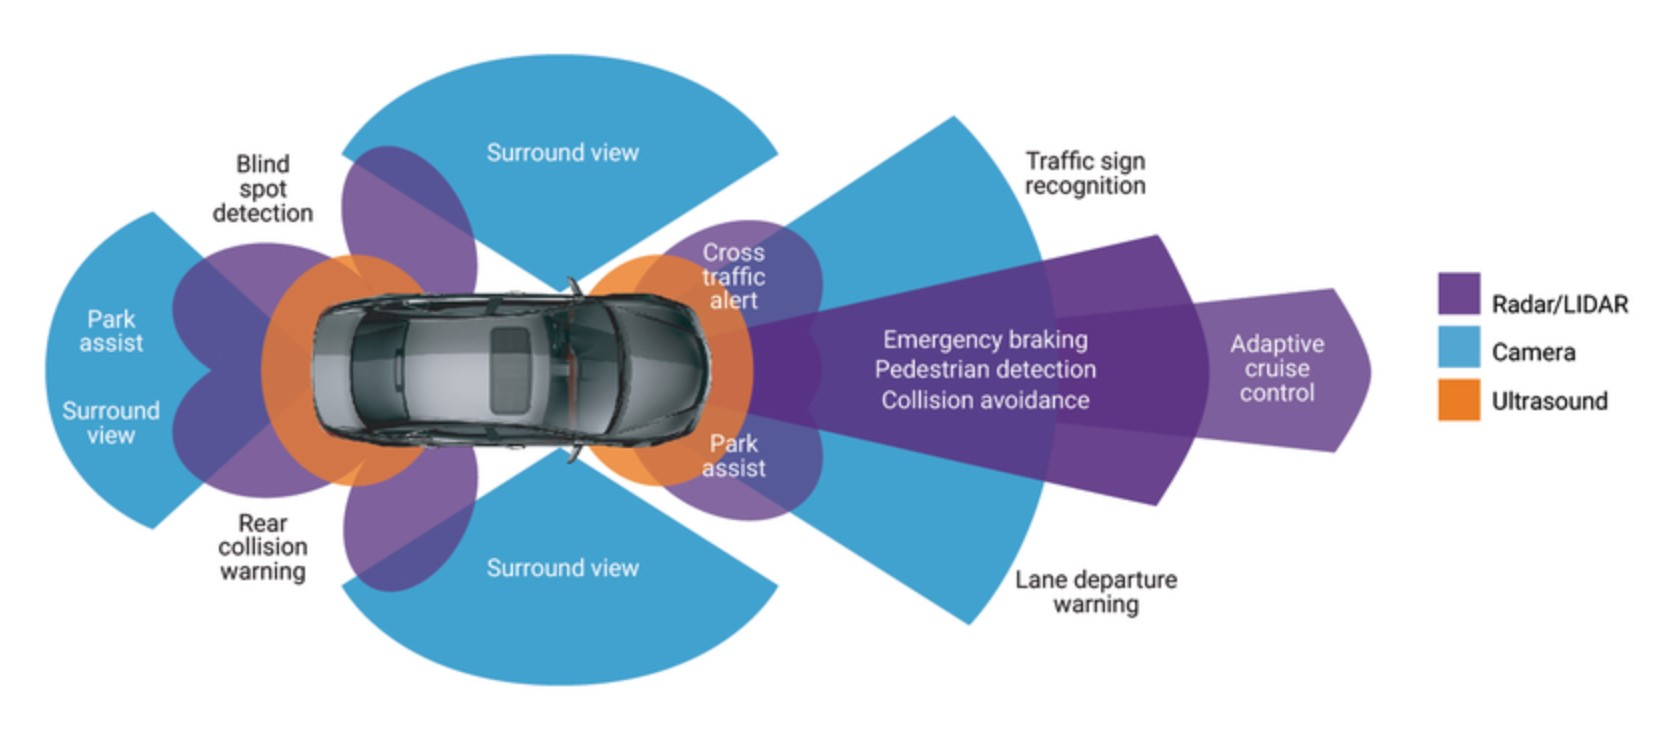
\includegraphics[width=0.95\textwidth]{Implementation-of-ADAS.jpg}
    \caption{Multi-sensor coverage and functional mapping in a Level-2 \ac{ADAS}.}
  \label{fig:multi-sensor-adas}
\end{figure}

Modern \ac{ADAS} utilize a set of diverse sensors in order to provide a robust perception environment as depicted in Figure~\ref{fig:multi-sensor-adas}. By fusing complementary sensing modalities that compensate for the limitations of individual sensors, improving reliability in varying light, weather, and traffic settings. Camera-based systems continue to occupy a prominent position and vary in complexity, such as in Tesla Autopilot and multi-camera systems in Waymo, which provide nearly 360° coverage \cite{ref11, ref10}. Monocular systems are relatively inexpensive and efficient in computation but not able to provide depth information and are susceptible to variations in illumination. The stereo and multi-camera approaches can overcome these problems through geometric reasoning but are more computationally expensive and challenging in terms of calibration procedures \cite{ref12}.

\ac{LiDAR} sensors are complementary to vision sensors as these sensors enable precise three-dimensional geometric measurements irrespective of the environment lighting conditions. Though initial autonomous vehicles use \ac{LiDAR} systems with mechanically rotating \ac{LiDAR} devices, nowadays solid-state \ac{LiDAR} configuration systems are dominating due to reliability and automotive adaptability issues \cite{ref14}. The millimeter wave radar sensor further adds reliability as it offers precise range and relative velocity measurement irrespective of deterioration due to harsh environmental conditions that degrade optical sensors and are essential for \ac{SAE} Level-2 \ac{ACC} functions \cite{ref12}.

Accurate spatial and temporal calibration is crucial for effective multi-sensor perception. Hardware-synchronized acquisition combined with precise timestamping allows for proper fusion, while in-vehicle networks like CAN support real-time control with latency low enough for most safety functions \cite{ref13}.
\subsection{Perception and Computer Vision}

Vision-based perception provides a basis for modern \ac{ADAS} technology, supporting detection, recognition, tracking, and free-space analysis. Lane detection began from classical image processing methods. However, the recent trends in image processing apply Deep Learning methods to image analysis tasks, including image detection. Convolutional neural networks have been proven to offer high resistance to normal working conditions \cite{ref12}. Semantic segmentation methods offer a pixel-level analysis of the environment, thereby supporting accurate detection for drivable regions.

Object detection in automotive applications favors systems which offer a better compromise between real-time performance and accuracy. Single-stage detectors gain popularity as they provide a more desirable trade-off between latency and error rate compared to their safety-critical counterparts, which usually employ redundancy to enhance robustness \cite{ref12}. The perception software stack provided by Tesla is a great example of a multi-task learning framework, which handles multiple tasks like object detection, segmentation, and depth prediction in a single network to enhance computational efficiency \cite{ref11}.

Multi-object tracking fuses perception outputs with motion models, providing essential temporal consistency for trajectory forecasting and collision avoidance. Most production and research methods rely on the tracking-by-detection paradigm, where learned appearance features are combined with probabilistic motion models \cite{ref12}. While great progress has been made, perception systems are still sensitive to dataset bias and domain shifts when the models of interest, so to say-trained in simulation or limited geographical areas-are tested in the real world, which requires continuous validation and sim-to-real adaptation.
\subsection{Path Planning and Decision Making}

Path planning and decision making form the core cognitive functions of autonomous vehicles, enabling them to navigate from origin to destination while ensuring safety, comfort, and efficiency. These functions are typically structured in a hierarchical framework comprising four key layers:

\begin{itemize}
    \item \textbf{Global Planning:} Determines overall route from start to destination based on road networks, traffic, and user preferences. Generates a coarse path without considering dynamic obstacles or real-time traffic.
    \item \textbf{Behavior Planning:} Tactical layer making high-level decisions about lane changes, overtaking, merging, and intersections.
    \item \textbf{Local Path Planning:} Operational level, generating collision-free trajectories within the immediate environment. Accounts for dynamic obstacles, road boundaries, and kinematic constraints.
    \item \textbf{Motion Prediction:} Forecasts trajectories of surrounding dynamic objects, enabling proactive planning and safer decision-making.
\end{itemize}

\paragraph{Automation Framework and Scope:}

The \ac{SAE} J3016 standard defines where strategic actions such as destination decision-making, trip planning, and waypoint decision-making are outside the scope defined by automation levels 0-5 and instead focuses on driving automation at a tactical and operational level defined by planning, local path planning, and motion prediction\cite{ref1}. Modern research endeavors on autonomous vehicles cover these operation defined levels using hierarchical architectures which encompass decision-making algorithms and real-time sensor processing abilities.


\paragraph{Behavior Planning and Decision Making:}

FSM architectures demonstrated effectiveness in multi-agent avoidance scenarios; Naranjo et al. achieved 50Hz real-time performance on Jetson-equivalent hardware \cite{ref16}. Decision tree methodologies provide structured behavior selection; Xu et al. integrated \ac{LiDAR}-camera fusion for motion prediction \cite{ref17}.

\paragraph{Path Planning Methodologies:}

Spline-based approaches have recently become quite popular for human-aware navigation in mixed traffic. Schörner et al. \cite{ref18} integrated the principles of Social Value Orientation into human-aware trajectory generation by using camera-\ac{LiDAR} fusion that enables dynamic obstacle handling at 20Hz on Jetson Nano platforms. The employment of quintic splines in their work guarantees smoothness in trajectories and real-time feasibility while accounting for social interactions.

The advantage of optimization-based methods is that they allow adaptability in dynamic environments. Reitmann et al. \cite{ref19} used Timed Elastic Bands after coarse A* planning, allowing fusion of single-camera and 3D \ac{LiDAR} for obstacle prediction. The real-time performance of the proposed approach surpasses 30Hz on Jetson Orin Nano hardware; it allows path density adjustment, hence scalable to embedded systems.
\paragraph{Motion Prediction and Trajectory Optimization}

Motion prediction systems utilize Kalman-filtered sensor fusion of camera point cloud data with \ac{LiDAR} data. Yeong et al. \cite{ref20} have shown that trajectory optimization using polynomial curves and reinforcement learning hybrids for decision-making in behavioral modeling can process sensor fusion in real time in under 50ms per layer on embedded GPU systems such as Jetson. The incorporation of reinforcement learning allows for adaptive decision-making-learning from experience.

More recently, Reachable Set Model Predictive Path Integral control methods were proposed for trajectory optimization. Liu et al. \cite{ref21} showed that by utilizing \ac{LiDAR} and camera occupancy grid predictions, collision-free polynomial splines can be obtained at real-time rates of 25 Hz for Orin Nano-scale hardware. This work has been identified as state-of-the-art in computationally efficient path planning.
\subsection{Control Systems}

\subsubsection{MPC/PID controllers for longitudinal and lateral control}

In the development of L2 autonomous systems, the "Adaptive Cruise Control" layer is responsible for translating perception data into physical vehicle actions.

This is split into \textbf{longitudinal control} (acceleration and braking) and \textbf{lateral control} (steering).

\begin{itemize}
    \item \textbf{Tesla} is moving their Full Self-Driving stack towards a Model Predictive Control solution.
    \item \textbf{GM employs MPC} in their Adaptive Cruise Control system to accomplish "eco-driving" objectives. Moreover, GM adopts robust control architecture combining map-based feed-forward control and MPC to provide high-fidelity lane centring control.
    \item \textbf{Ford's BlueCruise} has traditionally utilized a very sophisticated PID (Proportional Integral and Derivative) feedback control loop with feed-forward compensation for its Intelligent Adaptive Cruise Control.
\end{itemize}

PID is a reactive controller because it continually checks the error between current and desired states and takes steps to correct it only after it has happened. It is useful in Level 2 systems because it still involves human observation as a major component. On the other hand, MPC is optimal because it looks ahead into the future based on a time horizon and, in effect, foresees what is ahead on the road. Its ability to see ahead into potential road obstacles such as curves, traffic, and other objects makes it crucial to the decision-making process needed by advanced autopilot systems. \cite{ref6, ref7, ref8, ref9}

\subsubsection{Lane Keeping Assistant and Lane Centring Control}

In the hierarchy of driving automation, lateral control is divided into two primary categories: reactive systems that prevent lane departure and proactive systems that maintain a continuous path within the lane.

\begin{itemize}
    \item \textbf{Lane Keeping Assist:} This is a reactive safety feature that takes effect only when the car is about to cross lane markings without the turn signal on; it is an SAE Level 0-1 feature. It issues a rapid steering correction to push the car back into the lane.
    \item \textbf{Lane Centring Control:} Unlike LKA, this system continuously keeps the car centred in the lane through constant steering adjustments of minute nature. It is a key ingredient in Level 2 autonomous systems from Ford BlueCruise to GM Super Cruise, where it works in conjunction with Adaptive Cruise Control to maintain lane position and speed.
    \item \textbf{PID Control:} Simple, reliable, and easy to implement, with limited computing power. However, it is generally only reactive; it corrects the error after the error has occurred rather than planning ahead of it.
    \item \textbf{Model Predictive Control:} Now becoming the standard approach for advanced self-driving due to its capability of "looking ahead" and planning a trajectory in an optimal way regarding all upcoming curves, obstacles, and other constraints. It results in smoother driving, but requiring more computational power than PID. \cite{ref8, ref9, ref22}
\end{itemize}

\subsection{Level 2 Autonomous Systems Integration in Electric Vehicles}

The incorporation of SAE Level 2 autonomous systems in electric vehicles' platforms comes with its own set of technical considerations. The electric vehicle platform properties, such as torque response, regenerative braking, and their battery capacity, significantly affect the design of an autonomous system, demanding different strategies for control incorporation, energy management, and CPU allocation.

\subsubsection{Regenerative Braking Integration with Autonomous Control}

The integration of functionalities such as ACC and emergency brakes according to SAE Level 2 in electric cars needs smooth interfacing with regenerative brakes. The autonomous system needs to be able to manage deceleration actions along with the motor's capability for energy regeneration for maximizing deceleration and ensuring comfort and safety simultaneously. AI-based algorithms contribute to a braking time decrease of 11.5\% and also improve state-of-charge value by 0.487\% over traditional friction brakes \cite{ref23}. The algorithmic requirement is to be able to mix regenerative brakes and friction brakes real-time when performing emergency brakes and maximize deceleration at the cost of efficiency.

\subsubsection{Energy-Efficient Path Planning and Eco-Driving Strategies}

SAE Level 2 systems operating in electric vehicles can apply energy-conscious control strategies, thus improving the vehicle's range. Research has indicated that optimal energy prediction yields 6.3\% improvements in error margins for energy consumption estimations \cite{ref24}. When considering highway operating conditions in which Level 2 systems perform well, control strategies in Model Predictive Cruise Control utilize predictions regarding grade changes and traffic conditions in order to reduce energy consumption while satisfying time constraints specified by the driver.

\subsubsection{Battery Management Considerations for Compute-Intensive AI Workloads}

The use of SAE Level 2 perception and planning software in electric cars introduces competition for resource allocation in utilizing the battery power in electric cars. The edge computing modules involved in processing camera-based object detection and processing of LiDAR and other sensors consume 200-500W of power constantly \cite{ref25}. The resource-intensive processing power results in mileage losses of up to 5-10\%, depending on the operation being performed. Battery thermal management becomes critical as simultaneous fast charging and compute-intensive autonomous operations can accelerate cell degradation. Intelligent power management strategies dynamically adjust algorithm complexity based on battery state, thermal conditions, and scenario criticality.

\subsubsection{Vehicle Dynamics Modeling for Electric Powertrains}

Lane centering and trajectory tracking at Level 2 on electric vehicles need adapted control models that account for the electric powertrain dynamics. Electric motors provide instantaneous torque without lag, enabling precise lateral control but requiring different stability management compared to internal combustion vehicles. The placement of the batteries changes the weight distribution and, consequently, the center of gravity, altering the characteristics of the handling that the autonomous controllers must accommodate. Energy-efficient model predictive control approaches optimize motor torque delivery across driving phases, demonstrating 11.74\% improvement in energy recovery while maintaining Level 2 performance requirements \cite{ref26}.

\subsection{Safety and Validation}

SAE Level 2 autonomous vehicles development implies the incorporation of safety standards and validation methodologies, together with practical road testing protocols. This review examines functional safety frameworks, simulation-based testing, and critical safety mechanisms for reliable implementation using embedded platforms like NVIDIA Jetson with camera and LiDAR sensors.

\subsubsection{Functional Safety Standards}

For the safety of autonomous vehicles, two different ISO guidelines work in conjunction for safety. ISO 26262 provides a safety life cycle in the form of ASIL requirements for electrical/electronic systems in automobiles. ISO 21448, or SOTIF, deals with the safety risks that result in situations where the system does not fail but ignores situations such as an icy road when operating systems that rely on sensors \cite{ref27}. Together, these standards ensure comprehensive safety coverage against malfunctions and performance limitations for camera-LiDAR configurations.

\subsubsection{Simulation-Based Validation}

Validation on a virtual simulation platform precedes road testing. Engineers subject embedded system chips to diverse scenarios, such as uncommon and critical situations, with platforms like CARLA, LGSVL, and PreScan. Test conditions are determined by operational design domain (ODD), object detectability, and failure modes. In AEB system validation, Euro NCAP protocols require TTC measures with critical limits set to TTC $<$ 2.5 seconds for emergency action \cite{ref28}.

\subsubsection{Operational Design Domain and Safety Validation}

ODD identifies conditions under which the autonomous system can be operated without risk of harm, such as scenarios on highways under typical weather conditions but with challenges under adverse scenarios. SOTIF analysis of validations uses "combinatorial methods and Monte Carlo sampling" for analyzing failure rates of less than $10^{-9}$ in one hour to satisfy ODD boundaries \cite{ref29}. For camera and LiDAR systems, it involves validating performance under conditions of sensor occlusion, weather conditions, lighting conditions, and edge cases on operation boundaries.

\subsubsection{Road Testing Safety Mechanisms}

During on-road testing of SAE Level 2 systems, test personnel and road users are protected by several layers of safety. First, there is a licensed safety driver who must be "continuously attentive to the traveled way, completely alert, and ready to take control of the vehicle with latency between 4-10 seconds when the driver is alerted to system limitations". Emergency stop functions include easy-to-reach kill switches that shut off autonomous operation in an instant. Vehicles are also required to capture and store sensor data up to at least 30 seconds before the moment of any collision \cite{ref30}.

\subsubsection{Safety Architecture and Runtime Monitoring}

Jetson-based systems are required to have redundant sensor fusion through Kalman filtering to maintain functionality even if sensors fail, and fail-operational planning modules are used to provide safe trajectories in systems that have partial failures. Edge computing is used, which involves processing data on vehicles, reducing the processing time, and is even up to 2 GB/s \cite{ref25}.

SAE Level 2 requires eye-tracking and hand-wheel observation to ensure the preparedness of the system to take control. A clean human-machine interface helps in easy communication with proper system status and escalating warning cascades to avoid over-reliance on automated control.

There is hardware-based monitoring independent of the software program state through watchdog timer implementations, which issue resets upon the loss of periodic refresh pulses. For the NVIDIA Jetson-series of platforms, nested watchdog techniques integrating timer support in the Linux kernel and at the level of the bootloader offer fail-safe capability, which is able to detect stalled algorithms in hundreds of milliseconds, while the watchdogs in the firmware prevent kernel panics by automatically switching the boot slot. This design is able to support the requirements of independent monitoring of safety-critical tasks as specified by the ISO 26262 standard.
\section{Gaps in Literature}

While the existing literature provides substantial foundations for autonomous vehicle development, several gaps remain relevant to the present project:

\begin{itemize}
    \item \textbf{Limited Sim-to-Real Validation in Urban Scenarios:} Most published sim-to-real transfer research focuses on highway or simple track environments. Comprehensive validation of perception and control transfer in complex urban scenarios with pedestrians, traffic signals, and intersections remains limited, particularly for \ac{SAE} Level 2 systems operating at low speeds.
    
    \item \textbf{Resource-Constrained Multi-Sensor Fusion:} While sensor fusion techniques are well-documented for high-performance computing platforms, optimization strategies for real-time multi-modal fusion on embedded platforms like Jetson Orin remain under-explored, particularly when integrating camera and \ac{LiDAR} data for simultaneous object detection, lane keeping, and traffic signal recognition.
    
    \item \textbf{Adaptive Control Tuning for Retrofitted Platforms:} Most autonomous control research assumes purpose-built platforms with known dynamics. Methods for automatic identification and adaptation of control parameters for retrofitted electric vehicles with unknown or variable dynamics represent an important gap, as manual tuning is time-consuming and requires specialized expertise.
    
    \item \textbf{Integration of Multiple \ac{SAE} Level 2 Features:} While individual components of Level 2 systems (\ac{ACC}, \ac{LKA}) are extensively studied independently, research on their integrated operation, conflict resolution between subsystems, and seamless transitions between different automation modes is less comprehensive. The present project's holistic approach to implementing multiple Level 2 features simultaneously addresses this gap.
    
    \item \textbf{Low-Speed Urban Autonomy:} The majority of autonomous driving research targets highway scenarios or higher-speed operation. The specific challenges of low-speed urban autonomy (10--30 km/h), including frequent stop-start cycles, close-proximity obstacle avoidance, and interaction with vulnerable road users, receive less attention but are critical for practical urban deployment.
\end{itemize}

These gaps inform the research approach and expected contributions of the present project, particularly in demonstrating complete system integration from simulation through real-world deployment on a resource-constrained embedded platform operating in urban scenarios.

\chapter{Methodology}
\section{Research Design}

The autonomous vehicle system architecture follows a hierarchical decomposition consisting of four primary layers.

\begin{figure}[ht!]
    \centering
    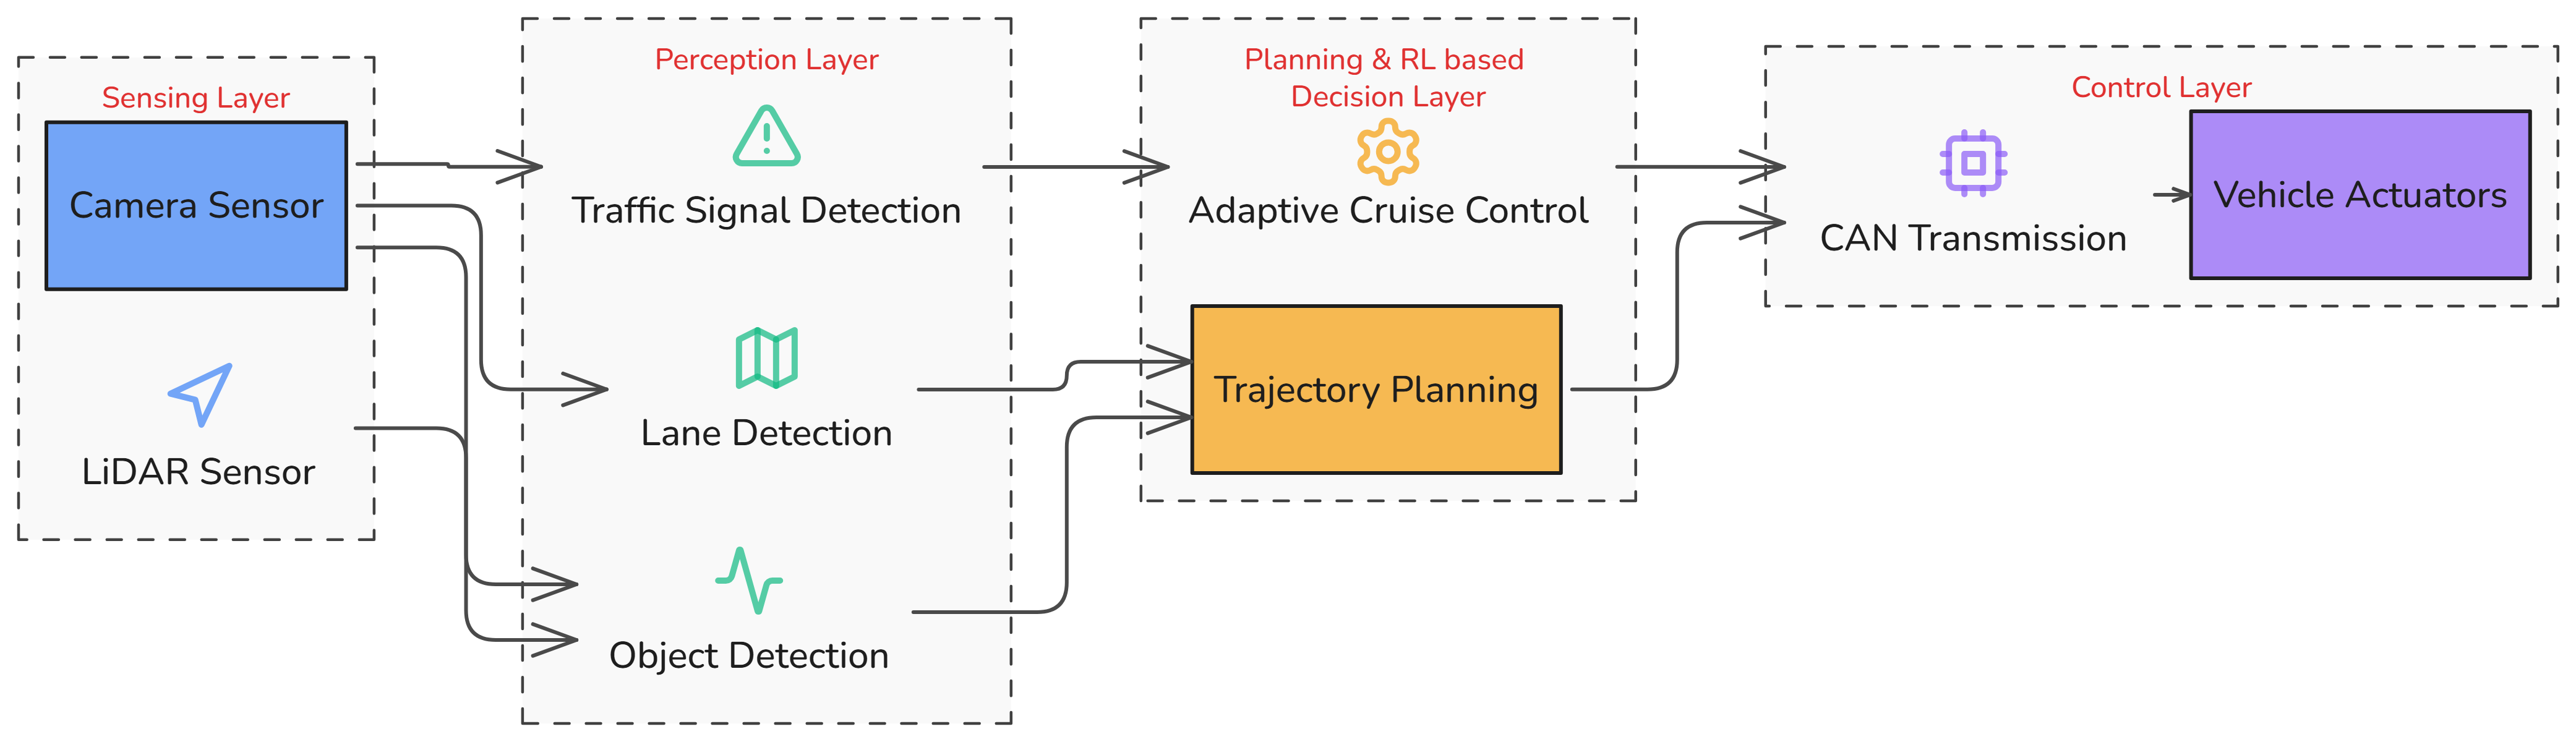
\includegraphics[width=0.95\textwidth]{ADAS-Architecture.png}
    \caption{Hierarchical autonomous vehicle system architecture showing the four primary layers: Sensing, Perception, Planning, and Control.}
    \label{fig:av-architecture}
\end{figure}

As shown in Figure \ref{fig:av-architecture}, the system consists of four distinct layers that process data from sensors to vehicle actuator commands.

\subsection{System Architecture}

\paragraph{Sensing Layer}

Physical sensors including a camera and \ac{LiDAR} acquire raw environmental data. This layer includes sensor drivers, calibration data, and low-level data preprocessing.

\paragraph{Perception Layer}

Processes sensor data to extract semantic information about the environment. Modules include object detection, lane detection, and traffic signal recognition \cite{ref19}. Outputs are represented as structured data describing detected entities, their properties, and spatial relationships.

\paragraph{Planning Layer}

Consumes perception outputs to generate vehicle behavior plans. Modules include trajectory planning, decision-making, and behavioral arbitration \cite{ref3,ref44}. Outputs consist of target trajectories expressed as sequences of waypoints with associated target speeds.

\paragraph{Control Layer}

Translates planned trajectories into vehicle actuator commands. Modules include lateral control (steering) and longitudinal control (throttle/brake) \cite{ref5}. The layer interfaces with vehicle drive-by-wire systems through standardized control messages.

A central data management component maintains system state, logs sensor data and algorithm outputs for offline analysis, and coordinates timing across modules to ensure synchronized operation.

\subsection{Simulation Environment Development}

\paragraph{Sensor Configuration}

Virtual sensors in \ac{CARLA} are configured to match the specifications of physical sensors used in hardware deployment. Camera parameters, including resolution, field of view, exposure, and mounting position, are matched to the Arducam specifications. \ac{LiDAR} configuration, including scan rate, vertical and horizontal resolution, range, and point density, is configured to represent the physical \ac{LiDAR} sensor.

\paragraph{Adaptive Cruise Control}

Adaptive Cruise Control is implemented by configuring longitudinal control logic in CARLA to replicate real-vehicle behavior, where radar-/\ac{LiDAR}-based lead vehicle detection, time headway thresholds, and acceleration–deceleration limits are matched to the constraints of the physical electric vehicle platform. Vehicle dynamics parameters, including maximum braking force, throttle response, and control update rate, are tuned to reflect the real drivetrain and actuator characteristics to ensure consistent speed regulation during simulation-to-hardware transfer.

\paragraph{Trajectory Planning and RL-Based Decision Making}

Trajectory planning and RL-based decision-making modules are trained in the \ac{CARLA} environment using vehicle kinematic constraints, lane geometry, and traffic interaction rules that closely approximate real-world operating conditions. The state space, action space, and reward function are designed to align with physical vehicle limits, ensuring that learned policies generate safe, feasible steering and speed commands when deployed on the real electric vehicle under supervised Level 2 autonomy.

\subsection{Perception Module Development}

\subsubsection{Object Detection}

\paragraph{LiDAR Integration}

\ac{LiDAR} point clouds are processed to identify clusters corresponding to potential obstacles \cite{ref4}. A voxel-based approach segments the point cloud, groups adjacent points into clusters, and fits bounding boxes to clusters. Camera detections and \ac{LiDAR} clusters are associated using spatial correspondence, with combined detections providing both semantic class information (from camera) and accurate 3D position (from \ac{LiDAR}).

\paragraph{Output Format}

Detections are published as a structured message containing object class, 2D bounding box coordinates, 3D position estimate, and confidence score. Detection rate targets 10 Hz minimum to enable responsive control.

\subsection{Lane Keeping Assistance Development}

The Lane Keeping Assistance system maintains vehicle position within the detected ego-lane through continuous steering adjustments \cite{ref33}. A cascaded control architecture is employed with separate controllers for lateral error and heading error.

\paragraph{Lateral Controller}

A PID controller minimizes lateral offset from the lane center. The controller input is the lateral distance (in meters) between the vehicle center and the detected lane center at a look-ahead distance (typically 10--15 meters). The controller output is a target steering angle.

\paragraph{Heading Controller}

A secondary PID controller minimizes heading error (angle between vehicle heading and lane direction). This controller improves tracking through curves and reduces oscillation around the lane center.

\paragraph{Control Fusion}

The final steering command combines outputs from lateral and heading controllers through weighted summation. Weights are tuned to achieve a critically damped response with minimal overshoot.

\paragraph{Speed Adaptation}

Controller gains are adapted based on vehicle speed, as steering response characteristics change with velocity. At lower speeds, higher gains provide more responsive correction, while at higher speeds, reduced gains prevent excessive control action.

\paragraph{Safety Limits}

Steering commands are limited to maximum rates and magnitudes compatible with vehicle kinematics and passenger comfort. If lane detection confidence drops below a threshold, the controller reduces gain or disengages entirely, alerting the driver to resume manual control.

\subsection{Trajectory Planning and Decision-Making Development}
\subsubsection{Planning and Decision-Making}

This module is charged with the responsibility of translating perception output on how safe and smooth vehicle motion should look like under Level 2 supervision. The proposed method adopts a hierarchical architecture that distinguishes between the decision-making and trajectory planning phases and is integrated in such a way that it is safe and real-time feasible.

\paragraph{Decision-Making Module}

This module analyzes and makes decisions regarding the current driving scenario to decide upon appropriate longitudinal driving maneuvers. It runs at a higher level of abstraction.

Key responsibilities include:

\begin{itemize}
    \item Identifying the current traffic context, such as free-flow driving, dense traffic, lead-vehicle following, or approaching traffic signals.
    \item Selecting the appropriate driving mode, including cruising, adaptive following, smooth deceleration, or full stop.
    \item Assessing risk levels associated with detected objects using perception outputs, including object class, distance, and relative velocity.
    \item Adapting safety margins such as time-gap and braking aggressiveness based on traffic density and perceived risk.
    \item Incorporating short-horizon motion prediction of surrounding vehicles to anticipate potential conflicts.
\end{itemize}

Decision-making is implemented using a hybrid approach:

\begin{itemize}
    \item Rule-based logic enforces traffic rules, safety constraints, and system operational limits.
    \item A reinforcement learning (RL) component is used for adaptive parameter tuning, particularly for time-gap adjustment and object risk scoring, without performing direct control actions.
\end{itemize}

The states of the agent are a compact state space including the speed of the ego vehicle, relative distance and velocity of lead vehicles, traffic density indicators, and signal states. The objectives of the reward function are to maximize safety, smoothness, and efficacy, while discouraging aggressive acceleration, unsafe gap acceptance, and unnecessary stops.

\subsection{Trajectory Planning Module}

The trajectory planning module generates a feasible and smooth longitudinal trajectory based on the selected driving mode and safety parameters provided by the decision-making layer.

Key responsibilities include:

\begin{itemize}
    \item Generating target speed profiles along the ego-lane that maintain safe following distances and comply with traffic signals.
    \item Ensuring smooth transitions between acceleration, cruising, and deceleration to enhance passenger comfort.
    \item Respecting vehicle dynamic limits, including acceleration, jerk, and braking constraints.
    \item Adjusting trajectory optimization cost weights based on risk levels supplied by the decision-making module, where higher perceived risk increases penalties on speed, acceleration, and proximity to obstacles, resulting in more cautious and conservative motion profiles.
\end{itemize}

Trajectory planning is formulated as a local planning problem and implemented using:

\begin{itemize}
    \item Lane-centerline-based planning for Level 2 operation.
    \item Polynomial or spline-based trajectory generation to ensure continuity in velocity and acceleration.
    \item Model Predictive Control (MPC) for longitudinal trajectory optimization over a receding horizon, enabling real-time adjustment to dynamic traffic conditions.
\end{itemize}

\paragraph{Integration with Adaptive Cruise Control}

The result from the trajectory planning module is the target speed and acceleration to the Adaptive Cruise Control (ACC) module. This is followed by the execution of the targets from the ACC module while ensuring a safe distance from the preceding vehicles as well as traffic signals.

Hierarchical decentralization of decision-making tasks and trajectory planning reduces modularity issues, interpretability, and validation of security by incorporating elements of learnability that do not deteriorate deterministic control scenarios.
\subsection{Adaptive Cruise Control Development}

The Adaptive Cruise Control (ACC) system regulates vehicle speed to maintain safe following distances from lead vehicles while tracking a driver-specified target speed when no lead vehicle is present \cite{ref1,ref32}.

\paragraph{Lead Vehicle Tracking}

Object detection and LiDAR data are fused to identify vehicles in the ego-lane ahead of the autonomous vehicle. A Kalman filter tracks lead vehicle position and velocity, providing filtered estimates that reduce sensor noise.

\paragraph{Following Distance Policy}

Safe following distance is computed using a time-gap policy where the target gap is proportional to current vehicle speed (typically 2--3 seconds). This approach naturally increases following distance at higher speeds while maintaining closer gaps at low speeds.

\paragraph{Longitudinal Control}

A Model Predictive Control (MPC) approach is employed for longitudinal control \cite{ref32}, optimizing the predicted vehicle trajectory over a receding horizon (typically 2--3 seconds). The optimization objective balances tracking target speed, maintaining a safe gap to the lead vehicle, passenger comfort (limiting acceleration and jerk), and fuel efficiency.

\paragraph{Deceleration for Traffic Signals}

When a red traffic signal is detected, the ACC system computes the required deceleration to stop at the signal stop line. Deceleration is applied smoothly beginning at a distance that allows comfortable braking rates (typically 2--3 m/s$^2$).

\paragraph{Speed Limits and Curvature}

The ACC system respects speed limits detected from traffic sign recognition and reduces speed for sharp curves based on estimated curve radius and assumed lateral acceleration limits \cite{ref40}.

\subsection{Testing and Validation Methodology}

\paragraph{Functional Validation}

An initial validation phase evaluates perception, decision-making, trajectory planning, and control algorithms in a fully controlled and repeatable environment. This stage enables systematic testing across a wide range of predefined scenarios, allowing verification of logical correctness, algorithm stability, and baseline performance without exposure to real-world risks.

\paragraph{Level 2 Performance Benchmarks}

System performance is evaluated against quantitative benchmarks aligned with Level 2 operational requirements:

\begin{itemize}
    \item Lane keeping performance: mean lateral deviation less than 0.2 m and maximum deviation less than 0.5 m.
    \item Speed regulation accuracy: steady-state speed error maintained within 5\% of target speed.
    \item Emergency response capability: reaction time less than 2 seconds for obstacle detection and deceleration initiation.
    \item System latency: end-to-end perception-to-control latency below 100 ms.
    \item System availability: operational uptime greater than 95\% within the defined operational design domain.
\end{itemize}

\paragraph{Operational Scenario Evaluation}

Once basic functionality is validated, testing advances to operational scenarios representative of the target deployment environment. Testing occurs during daytime, clear weather conditions on roads with visible lane markings, matching the defined operational design domain.

\chapter{Timeline and Resource Required}

\section{Timeline}
\subsection{7\textsuperscript{th} Semester (December 2025 - April 2026)}
\label{subsec:semester7}

\begin{table}[H]
\centering
\caption{Timeline of activities for the 7\textsuperscript{th} semester (December 2025 - April 2026)}
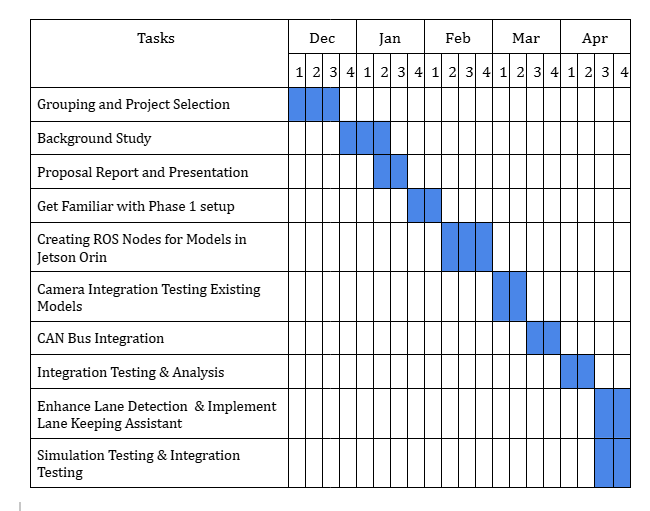
\includegraphics[width=0.95\textwidth]{semester7_timeline.png}
\label{tab:semester7_schedule}
\end{table}

\subsection{8\textsuperscript{th} Semester (May 2026 - September 2026)}
\label{subsec:semester8}

\begin{table}[H]
\centering
\caption{Timeline of activities for the 8\textsuperscript{th} semester (May 2026 - September 2026)}
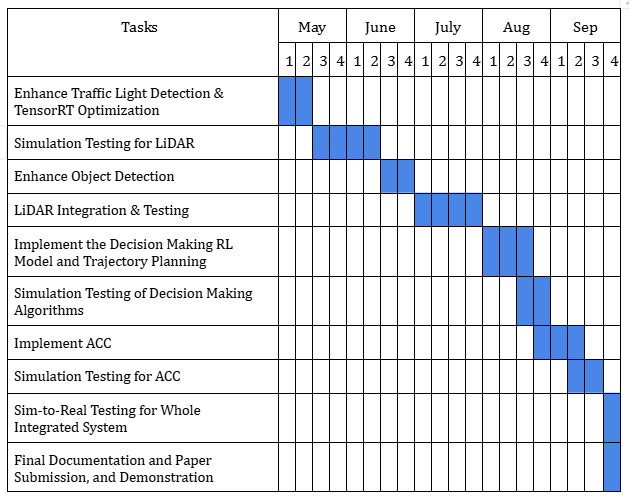
\includegraphics[width=0.95\textwidth]{semester8_timeline.png}
\label{tab:semester8_schedule}
\end{table}

\newpage

\section{Resources Required}

\paragraph{}
This section details the estimated cost allocation for physical implementation of SAE level 2 ADAS. The cost estimates below serve as a baseline to ensure that the project remains within budget during both development and deployment phases.

\begin{table}[h]
\centering
\caption{Estimated hardware expenditure for the development and validation of the proposed ADAS system}
\label{tab:hardware_cost}
\renewcommand{\arraystretch}{1.3}
\begin{tabular}{|p{4cm}|p{7cm}|p{3cm}|}
\hline
\textbf{Cost Item Hardware} & \textbf{Description} & \textbf{Cost (LKR)} \\ \hline

Arducam xISP - Swift AR0234 Camera &
2.3 MP global shutter camera used for lane detection, object detection, and traffic signal recognition. Compatible with NVIDIA Jetson platforms. &
Rs.\ 45,493.49 \\ \hline

MCP2515 CAN Controller &
SPI-based CAN controller module for interfacing Jetson with vehicle ECU and drive-by-wire system. &
Rs.\ 400.00 \\ \hline

Assembled EV vehicle chassis &
EV platform with motor, steering, battery, and frame for SAE Level-2 ADAS integration. &
Rs.\ 1,145,020.80 \\ \hline

LiDAR &
Used for depth estimation, obstacle detection, and sensor fusion (LiDAR + camera) in ACC and collision avoidance. &
Rs.\ 185,725.92 \\ \hline

Jetson Orin Nano &
Edge AI computing unit for real-time perception, planning, and control using ROS~2. &
Rs.\ 77,000.00 \\ \hline

MicroSDXC (SD 3.0) &
Bootable 64 GB microSDXC storage with UHS-I speed class used as the primary OS and data storage medium for the Jetson Orin Nano developer kit. &
Rs.\ 6,296.00 \\ \hline

Computing Resources &
High-performance workstation for CARLA simulation and model training. &
Rs.\ 556,868.22 \\ \hline

\end{tabular}
\end{table}


\chapter{Conclusion}

This project offers a transparent and modular approach for realizing a Level 2 automated driving assistance system catering specifically to urban scenarios. Based on an existing simulation-based Level 1 system developed in Phase I, Phase II enhances the system for supervised partial automation using reinforcement learning to enable and assist, but not replace, deterministic control decisions. The hierarchical architecture allows for easy separation and development along sensing and perception, planning and decision-making, and control functions, facilitating efficient development and integration testing. The perception layer combines camera and LiDAR inputs for reliable and semantic outputs corresponding to detection of objects, lanes, and traffic signals in the operational domain. Decision-making and planning are based on hierarchical planning utilizing rule-based safety planning and learning-based adaptation, and also utilize trajectory planning based on optimization techniques addressing safety, comfort, and optimization objectives. Reinforcement learning is constrained to adaptive parameter tuning to preserve predictability and safety. Model predictive control governs longitudinal and lateral dynamics through the adaptive cruise control module, ensuring smooth speed transitions and safe following behavior. Overall, the proposed Level 2 system offers a robust, safety-aware, and modular foundation for urban driving, with clearly defined operational limits and continuous driver supervision.
\section*{Expected Outcomes}

\begin{itemize}
    \item A functioning Level 2 autonomous system demonstrated on a real electric vehicle
    \item Open-source software frameworks enabling replication by other researchers
    \item Comprehensive datasets (simulation and real-world) for further research
    \item Validated methodologies for sim-to-real transfer in autonomous driving
    \item Publications contributing to RL deployment and safety assurance literature
\end{itemize}

This project positions our team at the forefront of autonomous vehicle innovation, combining rigorous engineering with cutting-edge AI research to advance the state-of-the-art in intelligent transportation systems.


% References
\renewcommand{\bibname}{References}
\bibliographystyle{ieeetr}
\addcontentsline{toc}{chapter}{References}
\bibliography{bibliography}

\end{document}